% LaTeX source for textbook ``ThinkCPP , a game perspective''
% Copyright (C) 2023  Lisa Patacchiola and Allen B Downey

\chapter{Iteration}
\index{iteration}

One of the things computers are often used for is the automation
of repetitive tasks.  Repeating identical or similar tasks without
making errors is something that computers do well and people do
poorly.

The
type of repetition we will be looking at now is called {\bf iteration}, and C++ provides
several language features that make it easier to write iterative
programs.

The three features we are going to look at are the {\tt while}
statement, the {\tt do-while} statement, and the {\tt for} statement. There are another features, like the for-each and ranged based for loop, that we will cover in another chapter.

\section{The {\tt while} statement}
\index{statement!while}
\index{loop!while}
\index{while statement}

Using a {\tt while} statement, we can write a countdown. What we would want to do is start with a certain number, then have the number go down (and print it out) while it is above zero. Then, print Blastoff!.

Here is pseudocode for that:
\begin{verbatim}
Set n to 3
WHILE n is more than zero
    print n
    subtract 1 from n
ENDWHILE
print "Blastoff!"
\end{verbatim}

Next, we can convert this to C++ code. It is not that much different than the pseudocode. Just like if statements, while statements use conditions to know when to continue and when to end. As long as the condition after the {\tt while} is true, the loop will continue to run. Once it is false, the loop will stop.

\begin{lstlisting}
  n = 3;
  while (n > 0) {
    std::cout << n << std::endl;
    n = n-1;
  }
  std::cout << "Blastoff!" << std::endl;
\end{lstlisting}
%
You can almost read a {\tt while} statement as if it were
English.  What this means is, ``While {\tt n} is greater than
zero, continue displaying the value of {\tt n} and then reducing
the value of {\tt n} by 1.  When you get to zero, output the
word `Blastoff!'''

This can be drawn as the following flowchart. 
\begin{figure}[h]
    \centering
    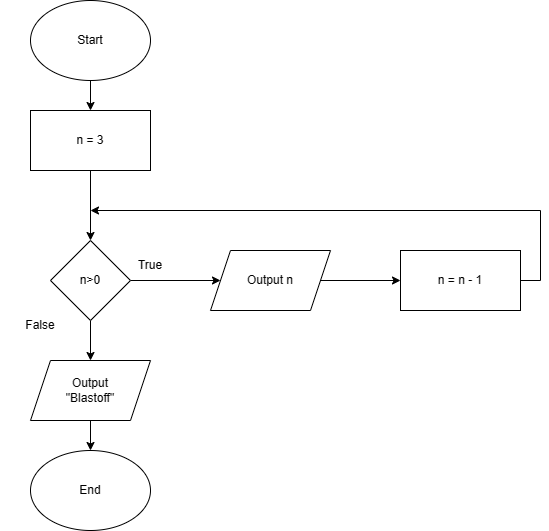
\includegraphics[width=9cm]{images/countdownwhileflow.png}
    \caption{Flowchart for the countdown program}
    \label{fig:countdownwhile}
\end{figure}
It is a little easier to understand how the code is looping by looking at the flowchart. Notice how after the n has one subtracted from it, the condition is checked again. That is the spot where it decides if the program will continue with the loop or end the loop.

More formally, the flow of execution for a {\tt while} statement
is as follows:

\begin{enumerate}

\item Evaluate the condition in parentheses, yielding {\tt true}
or {\tt false}.

\item If the condition is false, exit the {\tt while} statement
and continue execution at the next statement.

\item If the condition is true, execute each of the statements
between the curly-braces, and then go back to step 1.

\end{enumerate}

This type of flow is called a {\bf loop} because the third step loops
back around to the top.  Notice that if the condition is false the
first time through the loop, the statements inside the loop are
never executed.  The statements inside the loop are called
the {\bf body} of the loop.


\index{loop}
\index{loop!body}
\index{loop!infinite}
\index{body!loop}
\index{infinite loop}

The body of the loop should change the value of
one or more variables so that, eventually, the condition becomes
false and the loop terminates.  Otherwise the loop will repeat
forever, which is called an {\bf infinite loop}.  An endless
source of amusement for computer scientists is the observation
that the directions on shampoo, ``Lather, rinse, repeat,'' are
an infinite loop.

In the case of {\tt countdown}, we can prove that the loop
will terminate because we know that the value of {\tt n} is
finite, and we can see that the value of {\tt n} gets smaller
each time through the loop (each {\bf iteration}), so
eventually we have to get to zero.  In other cases it is not
so easy to tell:

\begin{verbatim}
    while (n != 1) {
      cout << n << endl;
      if (n%2 == 0) {           // n is even
        n = n / 2;
      } else {                  // n is odd
        n = n*3 + 1;
      }
    }

\end{verbatim}
%
The condition for this loop is {\tt n != 1}, so the loop
will continue until {\tt n} is 1, which will make the condition
false.

At each iteration, the program outputs the value of {\tt n} and then
checks whether it is even or odd.  If it is even, the value of
{\tt n} is divided by two.  If it is odd, the value is replaced
by $3n+1$.  For example, if the starting value (the argument passed
to {\tt sequence}) is 3, the resulting sequence is
3, 10, 5, 16, 8, 4, 2, 1.

Since {\tt n} sometimes increases and sometimes decreases, there is no
obvious proof that {\tt n} will ever reach 1, or that the program will
terminate.  For some particular values of {\tt n}, we can prove
termination.  For example, if the starting value is a power of two, then
the value of {\tt n} will be even every time through the loop, until
we get to 1.  The previous example ends with such a sequence,
starting with 16.

Particular values aside, the interesting question is whether
we can prove that this program terminates for {\em all} values of n.
So far, no one has been able to prove it {\em or} disprove it!

This book has a while loop simulator in order to help you understand while loops, \url{https://lpatacch.github.io/thinkCPPGamesEx/WhilePractice.html}. 
With this, you can change the 
initial value, the condition it is checking (\textless, \textgreater, ==, !=, \textgreater=, \textless=), the value checked,
and how the variable will change. Use this as many times as you wish
to understand how while loops work.
\section{New Operators}
Before we get more into loops, I want to cover some more math operators that we have not seen yet. In the countdown program, we had the counter change values with this equation:
\begin{verbatim}
    n = n-1;
\end{verbatim}
That equation took whatever was in n, subtracted 1, and placed it back in n. That behavior is very typical with loops. One variable 
is changed until it reaches the end value. It is so common that there is a short cut for this behavior. The above equation can be rewritten to this:
\begin{verbatim}
    n -= 1;
\end{verbatim}
This equation means the same as above, the value n has 1 subtracted from it, and then the result is put in n. Similar equations are available for many other math operators:
\begin{table}[h]
    \centering
    \begin{tabular}{|c|c|c|}
    \hline
 Math Operator & What it does & sample equation \\\hline
    +=     &  addition & {\tt n += 3;} \\
    -=      & subtraction & {\tt n -= 5;}\\
    {\tt *=}  &   multiplication & {\tt n *= 4;} \\
    \textbackslash=  &    division  & {\tt n \textbackslash= 2;}\\
    \%=  &  modulus & {\tt n \%= 7;}\\
\hline
    \end{tabular}
    \caption{New operators}
    \label{tab:newoperators}
\end{table}
\section{Increment and decrement operators}
\index{operator!increment}
\index{operator!decrement}

Incrementing and decrementing by one are such common operations that C++
provides special operators for them.  The {\tt ++} operator adds one
to the current value of an {\tt int}, {\tt char} or {\tt double}, and
{\tt --} subtracts one.  Neither operator works on {\tt string}s,
and neither {\em should} be used on {\tt bool}s.

The equation we modified in the last section:
\begin{verbatim}
    n -= 1;
\end{verbatim}

If you notice, the n was decremented by one. So, we can use the even shorter form here:
\begin{verbatim}
    --n;
\end{verbatim}
This subtracts 1 from n. This makes a very small line of code. All you need is the increment or the decrement operator, and the variable you will be changing.

You may have noticed that on some lines I put the ++ before the variable, and some after the variable. Both are legal. When it is on it's own line, it seems like it is doing the same thing. But, it is doing something slightly different. The ++ before the variable is called a pre-incrementor. It means that it will be doing the adding before anything else in the line. The ++ after the variable is called a post-incrementor. It means that it will be doing the adding after most of the things on the line. 

Technically, it is legal to increment a variable and use it
in an expression at the same time.  For example, you might see
something like:

\begin{verbatim}
  std::cout << i++ << std::endl;
\end{verbatim}
%
Looking at this, it is not clear whether the increment will
take effect before or after the value is displayed.  Because
expressions like this tend to be confusing, I would discourage
you from using them.  In fact, to discourage you even more,
I'm not going to tell you what the result is, other than letting you know it is a post-incrementor.  If you really
want to know, you can try it.

Using the increment operators, we can calculate the average weight of a person's inventory:

\begin{lstlisting}
  
  int num = 0;
  int weight = 0;
  int total = 0;
  std::cout << "Enter the weight of the item.\n"
  std::cout << "When done, enter -1\n";
  std::cin >> weight;
  while (weight >= 0) {
    //if it is a valid weight, add it to the total
    total += weight;
    
    //add one to the number of items
    ++num;
    
    //ask for the next weight
    std::cout << "Enter the weight of the item.\n"
    std::cout << "When done, enter -1\n";
    std::cin >> weight;    
  }
  
  if (num != 0)
  {
    std::cout << "The average is" << total/num <<".\n"; 
  }
  else {
    std::cout << "No items to average.\n";
  }
\end{lstlisting}
%
It is a common error to write something like

\begin{verbatim}
  num = num++;             // WRONG!!
\end{verbatim}
%
Unfortunately, this is syntactically legal, so the compiler
will not warn you.  The effect of this statement is to leave
the value of {\tt num} unchanged.  This is often a difficult
bug to track down.

Remember, you can write {\tt num = num +1;}, or you
can write {\tt num++;}, but you shouldn't mix them.

The ++ and -- does not work on a complex expression either. For example, 

\begin {verbatim}
( n + 7 )++;
\end{verbatim}
would not compile. The ++ and -- should be used only on a variable, not an expression.

\section{Parts of a loop}
The loops we have written so far have a number of elements
in common.  All of them start by initializing a variable;
they have a test, or condition, that depends on that variable;
and inside the loop they do something to that variable,
like increment it. This can be described by the following pseudocode:
\begin{verbatim}
  INITIALIZER;
  while (CONDITION) {
    BODY
    MODIFICATION
  }
\end{verbatim}
Loops, in order to work properly, need to have all three parts. If there is no modification section, the loop would never be able to leave the loop. If the initialization is wrong (or missing), the loop may loop the wrong amount of times (or never loop). And last, if the condition is wrong, the loop will never end properly. Whenever you loop is not working properly, if you look at those three parts, you will find the problem.

\section{Definite loop}
There are two different ways that loops can usually be identified. The first type 
is one where you know how many times the loop will repeat. These type of loops tend to
have a counter that is either counting down or up, and the counter is modified by a
constant value each time through the loop. These loops are sometimes called definite loops,
or counting loops. We have seen example with the countdown loop. The count down started at
three and the counter went down by one each time through the loop. Here is another example:

\begin{lstlisting}
  int val = 7;
  std::cout << "Here is a multiplication table for ";
  std::cout << val <<"\n";
  
  int x = 1;
  while (x <= 10)
  {
     std::cout << x << "\t" << x * val << "\n";
     x++;
  }
\end{lstlisting}
This loop has the condition as x<=10. If you look in the loop, you will notice that
x is being modified by 1 each time through the loop. Also, x is initialized to 1
when the loop starts. That means that the loop will repeat 10 times. Every time you
run this code, it will repeat 10 times.

In case you are interested, the \textbackslash t is one of the escape sequences that
we mentioned in \ref{tab:escapechar}. This spaces out each column by a tab stop. There 
are better ways to format tables, but we will not cover those methods for a while.

\section{Indefinite loop}
There is a different type of loop where you will not know how many times the loop
will run. The loop is checking a condition that will change, but it is different every
time we run the loop. We showed an example in the weight of the inventory code. This 
loop may have not repeated at all, or it could have repeated a thousand times. Since
you can not tell how many times it will repeat, it can be called an "indefinite loop". 
The number of repeats depended on what the user was entering. That code was waiting on a particular value (a negative number).
When a loop is waiting for a particular value, that value is called a flag, or a sentinel, which is why this loop may be
called a sentinel loop. 

\index{code blocks}
Just like if statements do not require curly braces to run, while loops don't either. A while loop without curly braces will only repeat the line right after the while condition. That is because the definition of a while loop is:

\begin{verbatim}
while (condition)
   statement or code block
\end{verbatim}

It is suggested that you always use code blocks with while loops to
prevent confusion and bugs.
\section{{\tt do-while} statement}
\index{statement!do-while}
\index{loop!do-while}
\index{do-while statement}
The second type of loop that C++ supports is called a do-while loop.
It works very similarly to the while loop. It should be initialized
before the loop starts, it should be modified inside the loop, and
it has a condition it checks. The difference is where it checks the
condition. The do-while loop checks the condition at the end of the
loop, guaranteeing the loop always runs at least once. The while loop
checks the condition at the beginning, which could mean the loop
might not run at all. The general syntax looks like the following:

\begin{verbatim}
  INITIALIZER;
   do {
    BODY
    MODIFICATION
  } while (CONDITION);
\end{verbatim}
%

For example, the multiplication table could be changed to a do-while:
\begin{lstlisting}
  int val = 7;
  std::cout << "Here is a multiplication table for ";
  std::cout << val <<"\n";
  
  int x = 1;
  do {
     std::cout << x << "\t" << x * val << "\n";
     x++;
  } while (x <= 10);
\end{lstlisting}
\begin{figure}[h]
    \centering
    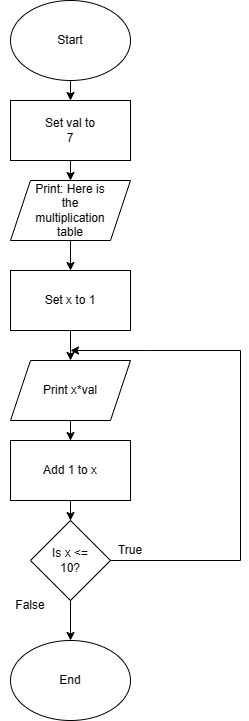
\includegraphics[height=10cm]{images/do-whileflow.png}
    \caption{Flowchart for the do-while multiplication table}
    \label{fig:do-while}
\end{figure}
By now, you may be wondering, "Why should I use this approach instead of a while loop?" The main advantage is that the code within the loop is guaranteed to execute at least once. I often use this type of loop when obtaining input from the user. In many programs, we ask a question. Unfortunately, the user may not always provide a valid response. While we know that we need to ask the question once, we cannot be certain if we will need to repeat it if the user provides an incorrect response. For instance, let's consider an example where we ask the user whether they want to turn left or right. The only correct answer is 'l' or 'r'. \footnote{Technically, we should have changed the answer to lowercase to allow for L and R,
but I wanted this example to be simpler than that.}
\begin{lstlisting}
  char direction = '\0';
  do {
     std::cout << "Do you want to go (l)eft or (r)ight?\n");
     std::cin >> direction;
     if ((direction != 'l')&&(direction != 'r'))
     {
        std::cout << "Please enter l or r\n";
     }
  } while ((direction != 'l')&&(direction != 'r'));
\end{lstlisting}
If we decided to do this with a while, we would have needed to ask 
the question both outside and inside the loop. The do-while reduces the amount of times the same code is duplicated in the program.

\section{{\tt for} statement}
\index{loop!for}
\index{for statement}
\index{statement!for}
We have had many examples of definite or counting loops.
This type of loop is so common that there is an alternate
loop statement, called {\tt for}, that expresses it more
concisely.  The general syntax looks like this:

\begin{verbatim}
  for (INITIALIZER; CONDITION; INCREMENTOR) {
    BODY
  }
\end{verbatim}
%
This statement is exactly equivalent to

\begin{verbatim}
  INITIALIZER;
  while (CONDITION) {
    BODY
    INCREMENTOR
  }
\end{verbatim}
%
except that it is more concise and, since it puts all the
loop-related statements in one place, it is easier to read.
For example:

\begin{verbatim}
  int i;
  for (i = 0; i < 4; i++) {
    cout << i << endl;
  }
\end{verbatim}
%
is equivalent to 

\begin{verbatim}
  int i = 0;
  while (i < 4) {
    cout << i << endl;
    i++;
  }
\end{verbatim}

Although using for loops when incrementing is common, it can
also be used when decrementing. Here is the countdown program
using a for loop instead:

\begin{lstlisting}
  for (n = 3; n > 0, n--) {
    std::cout << n << std::endl;
  }
  std::cout << "Blastoff!" << std::endl;
\end{lstlisting}

Also, the counter does not need to only change by one. You can use
any math operation that you want. Here is an example of a for loop
that modifies the counter by five every time through the loop.
\begin{lstlisting}
std::cout << "Counting to 100 by 5's \n";
for (n = 0; n < 100, n += 5 ) {
    std::cout << n << " ";
  }
std::cout << std::endl
\end{lstlisting}

\section{Break and Continue}
FIXME add examples of how this works
\section{Glossary}

\begin{description}

\item[loop:]  A statement that executes repeatedly while a
condition is true or until some condition is satisfied.

\item[infinite loop:]  A loop whose condition is always true.

\item[body:]  The statements inside the loop.

\item[iteration:]  One pass through (execution of) the body
of the loop, including the evaluation of the condition.

\item[definite loop:]  A loop where you know how many times
it will run before the loop starts.

\item[indefinite loop:]  A loop where you do not know how many
times it will run before the loop starts.


\index{loop}
\index{infinite loop}
\index{body}
\index{loop!infinite}
\index{iteration}


\end{description}

